\documentclass[12pt,a4paper]{article}
\usepackage{amsmath, amssymb, geometry, booktabs, xcolor, hyperref,
            listings, pgfplots, tcolorbox, enumitem, fancyhdr, tikz, array}
\geometry{margin=2.5cm}
\pgfplotsset{compat=1.18}
\tcbuselibrary{skins, breakable}

% ── tcolorbox environments ─────────────────────────────────────────────────
\newtcolorbox{curiositybox}[1]{colback=yellow!10, colframe=orange!80!black,
  fonttitle=\bfseries, title=#1, breakable}
\newtcolorbox{infobox}[1]{colback=blue!5, colframe=blue!60!black,
  fonttitle=\bfseries, title=#1, breakable}
\newtcolorbox{mistakebox}[1]{colback=red!5, colframe=red!60!black,
  fonttitle=\bfseries, title=#1, breakable}
\newtcolorbox{learnbox}[1]{colback=green!5, colframe=green!60!black,
  fonttitle=\bfseries, title=#1, breakable}

% ── lstlisting (Python) ────────────────────────────────────────────────────
\lstset{language=Python, basicstyle=\ttfamily\small, keywordstyle=\color{blue},
        commentstyle=\color{gray}, stringstyle=\color{orange},
        showstringspaces=false, numbers=left, numberstyle=\tiny,
        breaklines=true, frame=single}

% ── fancyhdr ──────────────────────────────────────────────────────────────
\pagestyle{fancy}
\fancyhf{}
\lhead{Topic 08: Laplace Transform of Derivatives}
\rhead{Unit IV --- Laplace Transforms}
\cfoot{\thepage}

% ── title ─────────────────────────────────────────────────────────────────
\title{Topic 08: Laplace Transform of Derivatives \\
       \large Unit IV --- Laplace Transforms}
\author{ \\
        JNTUA College of Engineering (Autonomous) ATP}
\date{}

% ==========================================================================
\begin{document}
\maketitle
\tableofcontents
\newpage

% ──────────────────────────────────────────────────────────────────────────
\section{Opening Hook}
% ──────────────────────────────────────────────────────────────────────────

\begin{curiositybox}{Hook}
You have been building a machine. Topic by topic, you assembled the
definition, the existence conditions, the standard table, the properties.
Now comes the moment the machine proves its worth. Take any ODE with
initial conditions --- say $y'' - 3y' + 2y = e^{4t}$, $y(0)=1$,
$y'(0)=0$. Apply the Laplace Transform to both sides. Every derivative
turns into a simple multiplication by $s$. The ODE becomes a linear
algebraic equation. Solve for $Y(s)$. Then invert. Done. No
characteristic equations, no undetermined coefficients. Just algebra.
This is why engineers love the Laplace Transform.
\end{curiositybox}

% ──────────────────────────────────────────────────────────────────────────
\section{Why This Topic Exists}
% ──────────────────────────────────────────────────────────────────────────

\textit{Before we begin, here is the honest answer to why you are reading
this\ldots}

Ordinary differential equations with initial conditions are the
bread-and-butter of engineering analysis. Every vibrating structure, every
electrical circuit, every control system is governed by ODEs. Classical
methods --- characteristic equation, variation of parameters, method of
undetermined coefficients --- are cumbersome when the forcing functions
are discontinuous, impulsive, or piecewise. The Laplace Transform
\emph{automates} the handling of initial conditions; they fall out of
the algebra automatically. No more hunting for particular solutions and
patching them with homogeneous solutions.

\medskip
\begin{center}
\begin{tabular}{@{}p{7cm}p{7cm}@{}}
\toprule
\textbf{Mistake} & \textbf{Consequence} \\
\midrule
Forgetting the initial condition terms in
$\mathcal{L}\{f'\}$ &
Losing the IC contribution and getting wrong ODE solutions \\
\midrule
Applying the formula without checking differentiability &
Getting incorrect results for non-smooth functions \\
\midrule
Not tracking which initial condition goes where in
$\mathcal{L}\{f''\}$ &
Swapping $f(0)$ and $f'(0)$ roles --- wrong final answer \\
\bottomrule
\end{tabular}
\end{center}

\begin{learnbox}{Key Takeaway}
The Laplace Transform converts an initial-value problem (IVP) into a
purely algebraic problem. Initial conditions are \emph{automatically
built into} the transformed equation --- there is no separate step to
impose them.
\end{learnbox}

% ──────────────────────────────────────────────────────────────────────────
\section{You Already Know This (Intuition First)}
% ──────────────────────────────────────────────────────────────────────────

Recall Fourier analysis: in the frequency domain of electrical
engineering, differentiation with respect to time becomes multiplication
by $j\omega$. This is exactly the same idea the Laplace Transform
exploits. The Laplace Transform takes the derivative $f'(t)$ and replaces
it with $sF(s)$ (minus an initial condition correction). It is not magic
--- it follows directly from integration by parts applied to the
definition integral
\[
  \mathcal{L}\{f(t)\} = \int_0^\infty e^{-st} f(t)\,dt.
\]
Think of $s$ as a ``frequency-like'' variable. Multiplying by $s$ in the
$s$-domain is the algebraic counterpart of differentiating once in the
$t$-domain. The initial condition term $f(0)$ is the ``memory'' of the
system at the starting instant --- it cannot be ignored.

% ──────────────────────────────────────────────────────────────────────────
\section{Transform of the First Derivative}
% ──────────────────────────────────────────────────────────────────────────

\begin{infobox}{Theorem: $\mathcal{L}\{f'(t)\}$}
\textbf{Statement.} Let $f(t)$ be continuous on $[0,\infty)$ and of
exponential order, and let $f'(t)$ be piecewise continuous on
$[0,\infty)$. Then
\[
  \boxed{\mathcal{L}\{f'(t)\} = s\,F(s) - f(0)}
\]
where $F(s) = \mathcal{L}\{f(t)\}$.

\medskip
\textbf{Proof by integration by parts.}

Start from the definition:
\[
  \mathcal{L}\{f'(t)\} = \int_0^\infty e^{-st}\,f'(t)\,dt.
\]
Choose $u = e^{-st}$ and $dv = f'(t)\,dt$, so $du = -s\,e^{-st}\,dt$
and $v = f(t)$. Integration by parts gives:
\[
  \int_0^\infty e^{-st}\,f'(t)\,dt
  = \Bigl[e^{-st}\,f(t)\Bigr]_0^\infty
    - \int_0^\infty (-s)\,e^{-st}\,f(t)\,dt.
\]
Evaluate the boundary term. Because $f(t)$ is of exponential order there
exists $M>0$ and $\sigma_0$ such that $|f(t)| \le M e^{\sigma_0 t}$ for
all large $t$. For $\text{Re}(s) > \sigma_0$:
\[
  \lim_{t\to\infty} e^{-st}\,f(t)
  \le \lim_{t\to\infty} M\,e^{-(s-\sigma_0)t} = 0.
\]
At $t=0$ the boundary term evaluates to $-e^{0}\,f(0) = -f(0)$.
Therefore:
\[
  \mathcal{L}\{f'(t)\}
  = \bigl(0 - f(0)\bigr) + s\int_0^\infty e^{-st}\,f(t)\,dt
  = -f(0) + s\,F(s)
  = s\,F(s) - f(0). \qed
\]
\end{infobox}

\begin{learnbox}{What Did We Learn?}
$\mathcal{L}\{f'(t)\} = s\,F(s) - f(0)$. Differentiation in the
$t$-domain $\longleftrightarrow$ multiplication by $s$ in the $s$-domain,
minus the value of the function at $t=0$.
\end{learnbox}

% ──────────────────────────────────────────────────────────────────────────
\section{Transform of the Second Derivative}
% ──────────────────────────────────────────────────────────────────────────

\begin{infobox}{Theorem: $\mathcal{L}\{f''(t)\}$}
\textbf{Statement.}
\[
  \boxed{\mathcal{L}\{f''(t)\} = s^2\,F(s) - s\,f(0) - f'(0)}
\]

\textbf{Derivation.} Treat $f''(t) = (f')'(t)$ and apply the first
derivative formula twice.

Let $g(t) = f'(t)$, so $g'(t) = f''(t)$.

Apply $\mathcal{L}\{g'(t)\} = s\,G(s) - g(0)$:
\[
  \mathcal{L}\{f''(t)\}
  = s\,\mathcal{L}\{f'(t)\} - f'(0).
\]
Now substitute $\mathcal{L}\{f'(t)\} = s\,F(s) - f(0)$:
\[
  \mathcal{L}\{f''(t)\}
  = s\bigl[s\,F(s) - f(0)\bigr] - f'(0)
  = s^2\,F(s) - s\,f(0) - f'(0). \qed
\]
\end{infobox}

\begin{learnbox}{What Did We Learn?}
Each additional derivative contributes one more power of $s$ and peels
off one more initial condition. $\mathcal{L}\{f''\} = s^2F(s) -
s\,f(0) - f'(0)$.
\end{learnbox}

% ──────────────────────────────────────────────────────────────────────────
\section{General \texorpdfstring{$n$}{n}th Derivative Formula}
% ──────────────────────────────────────────────────────────────────────────

\begin{infobox}{General Formula}
\textbf{Theorem.} If $f, f', \ldots, f^{(n-1)}$ are continuous on
$[0,\infty)$ and of exponential order, and $f^{(n)}$ is piecewise
continuous, then
\[
  \boxed{
    \mathcal{L}\{f^{(n)}(t)\}
    = s^n F(s)
    - s^{n-1}f(0)
    - s^{n-2}f'(0)
    - \cdots
    - s\,f^{(n-2)}(0)
    - f^{(n-1)}(0)
  }
\]

\medskip
\textbf{Proof by induction.}

\emph{Base case} ($n=1$): already proved --- $\mathcal{L}\{f'\} =
sF(s) - f(0)$. \checkmark

\emph{Inductive step}: assume the formula holds for $n=k$, i.e.,
\[
  \mathcal{L}\{f^{(k)}(t)\}
  = s^k F(s) - s^{k-1}f(0) - \cdots - f^{(k-1)}(0).
\]
For $n = k+1$, write $f^{(k+1)}(t) = \bigl(f^{(k)}\bigr)'(t)$ and apply
the first-derivative formula with $h(t) = f^{(k)}(t)$:
\[
  \mathcal{L}\{f^{(k+1)}(t)\}
  = s\,\mathcal{L}\{f^{(k)}(t)\} - f^{(k)}(0).
\]
Substitute the inductive hypothesis:
\[
  = s\bigl[s^k F(s) - s^{k-1}f(0) - \cdots - f^{(k-1)}(0)\bigr]
    - f^{(k)}(0)
  = s^{k+1}F(s) - s^k f(0) - \cdots - f^{(k)}(0). \qed
\]

\medskip
\textbf{Explicit $n=3$ case:}
\begin{align*}
  \mathcal{L}\{f'''(t)\}
  &= s\,\mathcal{L}\{f''(t)\} - f''(0) \\
  &= s\bigl[s^2 F(s) - s\,f(0) - f'(0)\bigr] - f''(0) \\
  &= s^3 F(s) - s^2 f(0) - s\,f'(0) - f''(0).
\end{align*}
\end{infobox}

\medskip
\begin{center}
\begin{tabular}{@{}c l@{}}
\toprule
$n$ & $\mathcal{L}\{f^{(n)}(t)\}$ \\
\midrule
1 & $s\,F(s) - f(0)$ \\
2 & $s^2 F(s) - s\,f(0) - f'(0)$ \\
3 & $s^3 F(s) - s^2 f(0) - s\,f'(0) - f''(0)$ \\
4 & $s^4 F(s) - s^3 f(0) - s^2 f'(0) - s\,f''(0) - f'''(0)$ \\
\bottomrule
\end{tabular}
\end{center}

\begin{learnbox}{What Did We Learn?}
The pattern is crystal clear: power of $s$ decreases by 1 for each
successive initial condition $f^{(k)}(0)$. For an $n$th-order ODE,
applying $\mathcal{L}$ produces an algebraic equation of degree $n$
in $s$ --- solvable by elementary algebra.
\end{learnbox}

% ──────────────────────────────────────────────────────────────────────────
\section{The ODE Solution Workflow}
% ──────────────────────────────────────────────────────────────────────────

\begin{infobox}{4-Step Workflow for Solving IVPs via Laplace Transforms}
\textbf{Step 1:} Apply $\mathcal{L}\{\cdot\}$ to \emph{both sides} of
the ODE. Use the derivative formulas to replace $y'$, $y''$, etc.\ by
algebraic expressions in $Y(s) = \mathcal{L}\{y(t)\}$.

\textbf{Step 2:} Substitute the numerical values of the initial
conditions $y(0)$, $y'(0)$, \ldots

\textbf{Step 3:} Collect and isolate $Y(s)$ --- solve the resulting
linear algebraic equation for $Y(s)$.

\textbf{Step 4:} Apply the inverse Laplace transform
$y(t) = \mathcal{L}^{-1}\{Y(s)\}$ using partial fractions and the
standard Laplace table to recover $y(t)$.
\end{infobox}

\medskip
\textbf{4-Step Workflow --- Block Diagram:}

\begin{center}
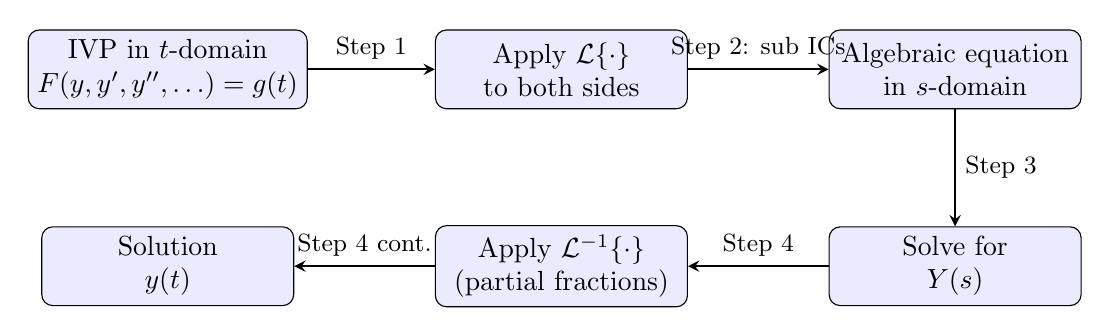
\begin{tikzpicture}[
    box/.style={draw, rounded corners, minimum width=3.2cm,
                minimum height=1cm, align=center, fill=blue!8},
    arr/.style={->, thick, >=stealth}
  ]
  \node[box] (A) at (0,0)   {IVP in $t$-domain\\$F(y,y',y'',\ldots)=g(t)$};
  \node[box] (B) at (5,0)   {Apply $\mathcal{L}\{\cdot\}$\\to both sides};
  \node[box] (C) at (10,0)  {Algebraic equation\\in $s$-domain};
  \node[box] (D) at (10,-2.5){Solve for\\$Y(s)$};
  \node[box] (E) at (5,-2.5) {Apply $\mathcal{L}^{-1}\{\cdot\}$\\(partial fractions)};
  \node[box] (F) at (0,-2.5) {Solution\\$y(t)$};

  \draw[arr] (A) -- node[above]{\small Step 1} (B);
  \draw[arr] (B) -- node[above]{\small Step 2: sub ICs} (C);
  \draw[arr] (C) -- node[right]{\small Step 3} (D);
  \draw[arr] (D) -- node[above]{\small Step 4} (E);
  \draw[arr] (E) -- node[above]{\small Step 4 cont.} (F);
\end{tikzpicture}
\end{center}

\begin{learnbox}{What Did We Learn?}
The four steps are mechanical: transform $\to$ substitute ICs $\to$
solve algebra $\to$ invert. Each step is elementary on its own; the
power comes from chaining them.
\end{learnbox}

% ──────────────────────────────────────────────────────────────────────────
\section{Worked Examples}
% ──────────────────────────────────────────────────────────────────────────

% ── Example 1 ─────────────────────────────────────────────────────────────
\begin{infobox}{Example 1 --- First-Order ODE: $y' + 2y = 4$, $y(0)=1$}
\textbf{Step 1: Apply $\mathcal{L}$ to both sides.}

$\mathcal{L}\{y' + 2y\} = \mathcal{L}\{4\}$

Using the first-derivative formula and linearity:
\[
  \bigl[s\,Y(s) - y(0)\bigr] + 2\,Y(s) = \frac{4}{s}.
\]

\textbf{Step 2: Substitute the initial condition $y(0)=1$.}
\[
  s\,Y(s) - 1 + 2\,Y(s) = \frac{4}{s}.
\]

\textbf{Step 3: Collect $Y(s)$.}
\[
  (s+2)\,Y(s) = \frac{4}{s} + 1 = \frac{4 + s}{s}.
\]
\[
  Y(s) = \frac{s+4}{s(s+2)}.
\]

\textbf{Step 4: Partial fractions.}

Write $\dfrac{s+4}{s(s+2)} = \dfrac{A}{s} + \dfrac{B}{s+2}$.

Multiply both sides by $s(s+2)$:
\[
  s + 4 = A(s+2) + B\,s.
\]
Set $s=0$: $4 = 2A \Rightarrow A = 2$.

Set $s=-2$: $2 = -2B \Rightarrow B = -1$.

Therefore:
\[
  Y(s) = \frac{2}{s} - \frac{1}{s+2}.
\]

\textbf{Step 5: Invert.}
\[
  y(t) = \mathcal{L}^{-1}\!\left\{\frac{2}{s}\right\}
         - \mathcal{L}^{-1}\!\left\{\frac{1}{s+2}\right\}
       = 2 - e^{-2t}.
\]

\textbf{Verification}: $y(0) = 2 - 1 = 1$ \checkmark.
$y'(t) = 2e^{-2t}$.
$y' + 2y = 2e^{-2t} + 2(2-e^{-2t}) = 2e^{-2t} + 4 - 2e^{-2t} = 4$
\checkmark.
\end{infobox}

\begin{learnbox}{What Did We Learn? (Example 1)}
For a first-order IVP, the Laplace method reduces to: one formula
application, one partial-fraction split, one table look-up. The initial
condition $y(0)=1$ was automatically incorporated in Step 2.
\end{learnbox}

% ── Example 2 ─────────────────────────────────────────────────────────────
\begin{infobox}{Example 2 --- Second-Order ODE: $y'' - 3y' + 2y = 0$, $y(0)=1$, $y'(0)=0$}
\textbf{Step 1: Apply $\mathcal{L}$ to both sides.}
\[
  \mathcal{L}\{y''\} - 3\,\mathcal{L}\{y'\} + 2\,\mathcal{L}\{y\} = 0.
\]

Expand each Laplace term:
\[
  \bigl[s^2 Y - s\,y(0) - y'(0)\bigr]
  - 3\bigl[s\,Y - y(0)\bigr]
  + 2\,Y = 0.
\]

\textbf{Step 2: Substitute $y(0)=1$, $y'(0)=0$.}
\[
  (s^2 Y - s - 0) - 3(s\,Y - 1) + 2\,Y = 0.
\]
\[
  s^2 Y - s - 3s\,Y + 3 + 2Y = 0.
\]

\textbf{Step 3: Collect $Y(s)$.}
\[
  (s^2 - 3s + 2)\,Y = s - 3.
\]
Factor: $s^2 - 3s + 2 = (s-1)(s-2)$.
\[
  Y(s) = \frac{s-3}{(s-1)(s-2)}.
\]

\textbf{Step 4: Partial fractions.}

Write $\dfrac{s-3}{(s-1)(s-2)} = \dfrac{A}{s-1} + \dfrac{B}{s-2}$.

Multiply both sides by $(s-1)(s-2)$:
\[
  s - 3 = A(s-2) + B(s-1).
\]
Set $s=1$: $-2 = -A \Rightarrow A = 2$.

Set $s=2$: $-1 = B \Rightarrow B = -1$.

Therefore:
\[
  Y(s) = \frac{2}{s-1} - \frac{1}{s-2}.
\]

\textbf{Step 5: Invert.}
\[
  y(t) = 2e^{t} - e^{2t}.
\]

\textbf{Verification}: $y(0) = 2-1 = 1$ \checkmark.
$y'(t) = 2e^t - 2e^{2t}$; $y'(0) = 2 - 2 = 0$ \checkmark.

$y'' - 3y' + 2y
 = (2e^t - 4e^{2t}) - 3(2e^t - 2e^{2t}) + 2(2e^t - e^{2t})
 = (2 - 6 + 4)e^t + (-4+6-2)e^{2t} = 0$ \checkmark.
\end{infobox}

\begin{learnbox}{What Did We Learn? (Example 2)}
A homogeneous second-order IVP is solved without guessing exponential
solutions. The characteristic roots $s=1$ and $s=2$ appear naturally as
the poles of $Y(s)$.
\end{learnbox}

% ── Example 3 ─────────────────────────────────────────────────────────────
\begin{infobox}{Example 3 --- Second-Order ODE with Forcing: $y'' + y = \cos t$, $y(0)=1$, $y'(0)=0$}
\textbf{Step 1: Apply $\mathcal{L}$ to both sides.}

Note $\mathcal{L}\{\cos t\} = \dfrac{s}{s^2+1}$.
\[
  \bigl[s^2 Y - s\,y(0) - y'(0)\bigr] + Y = \frac{s}{s^2+1}.
\]

\textbf{Step 2: Substitute $y(0)=1$, $y'(0)=0$.}
\[
  s^2 Y - s + Y = \frac{s}{s^2+1}.
\]
\[
  (s^2+1)\,Y = s + \frac{s}{s^2+1} = \frac{s(s^2+1)+s}{s^2+1}
             = \frac{s^3 + 2s}{s^2+1}.
\]

\textbf{Step 3: Solve for $Y(s)$.}
\[
  Y(s) = \frac{s^3 + 2s}{(s^2+1)^2}.
\]

\textbf{Step 4: Partial fractions over repeated irreducible quadratic.}

Write:
\[
  \frac{s^3+2s}{(s^2+1)^2}
  = \frac{As+B}{s^2+1} + \frac{Cs+D}{(s^2+1)^2}.
\]
Multiply both sides by $(s^2+1)^2$:
\[
  s^3+2s = (As+B)(s^2+1) + (Cs+D).
\]
Expand the right-hand side:
\[
  = As^3 + As + Bs^2 + B + Cs + D
  = As^3 + Bs^2 + (A+C)s + (B+D).
\]
Match coefficients:
\begin{align*}
  s^3 &: A = 1, \\
  s^2 &: B = 0, \\
  s^1 &: A + C = 2 \Rightarrow C = 1, \\
  s^0 &: B + D = 0 \Rightarrow D = 0.
\end{align*}
Therefore:
\[
  Y(s) = \frac{s}{s^2+1} + \frac{s}{(s^2+1)^2}.
\]

\textbf{Step 5: Invert.}

$\mathcal{L}^{-1}\!\left\{\dfrac{s}{s^2+1}\right\} = \cos t$.

For $\mathcal{L}^{-1}\!\left\{\dfrac{s}{(s^2+1)^2}\right\}$, use the
known result $\mathcal{L}\!\left\{\dfrac{t\sin t}{2}\right\} =
\dfrac{s}{(s^2+1)^2}$ (derivable via the $-dF/ds$ rule).

Therefore:
\[
  y(t) = \cos t + \tfrac{1}{2}\,t\sin t.
\]

\textbf{Verification}: $y(0) = 1+0 = 1$ \checkmark.
$y'(0) = (-\sin t + \tfrac{1}{2}\sin t + \tfrac{1}{2}t\cos t)\big|_{t=0}
= 0+0+0 = 0$ \checkmark.
\end{infobox}

\begin{learnbox}{What Did We Learn? (Example 3)}
Even when the forcing function $\cos t$ shares the natural frequency of
the system ($\omega = 1$), the Laplace method handles the resonance
algebraically: it appears as a repeated pole at $s = \pm i$ and produces
the $t\sin t$ term that is the hallmark of resonance.
\end{learnbox}

% ──────────────────────────────────────────────────────────────────────────
\section{pgfplots Visualization}
% ──────────────────────────────────────────────────────────────────────────

\textbf{Figure:} The solution $y(t) = 2 - e^{-2t}$ to Example 1,
showing the initial value $y(0)=1$ and the asymptote $y=2$.

\begin{center}
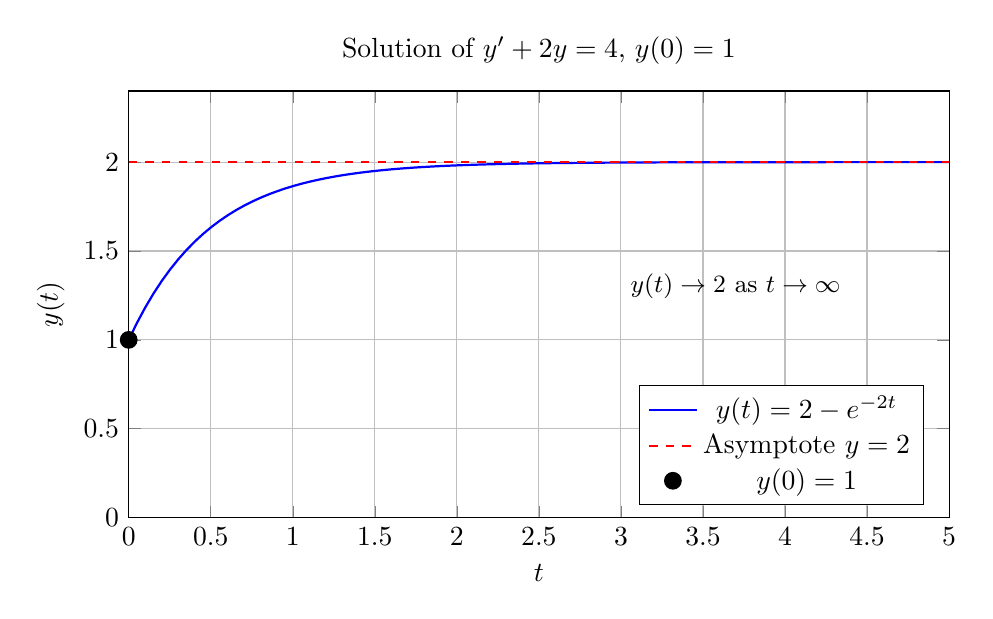
\begin{tikzpicture}
\begin{axis}[
  width=12cm, height=7cm,
  xlabel={$t$},
  ylabel={$y(t)$},
  xmin=0, xmax=5,
  ymin=0, ymax=2.4,
  grid=major,
  legend pos=south east,
  title={Solution of $y' + 2y = 4$, $y(0)=1$}
]
  % Solution curve
  \addplot[blue, thick, domain=0:5, samples=100]
    {2 - exp(-2*x)};
  \addlegendentry{$y(t)=2-e^{-2t}$}

  % Asymptote
  \addplot[red, dashed, thick, domain=0:5]
    {2};
  \addlegendentry{Asymptote $y=2$}

  % Initial value marker
  \addplot[only marks, mark=*, mark size=3pt, color=black]
    coordinates {(0,1)};
  \addlegendentry{$y(0)=1$}

  % Annotation
  \node[anchor=west] at (axis cs:3,1.3) {\small $y(t)\to 2$ as $t\to\infty$};
\end{axis}
\end{tikzpicture}
\end{center}

\textit{Caption: The Laplace method automatically incorporates the
initial condition $y(0)=1$ --- no need to impose it separately. The
solution rises smoothly from 1 toward the steady state 2.}

% ──────────────────────────────────────────────────────────────────────────
\section{Excel Example (Numerical Verification)}
% ──────────────────────────────────────────────────────────────────────────

We numerically verify $y(t) = 2 - e^{-2t}$ against an Euler-method
integration of $y' = 4 - 2y$, $y(0) = 1$, using step size $h = 0.1$.

\medskip
\begin{center}
\small
\begin{tabular}{@{} c c c c c @{}}
\toprule
\textbf{Col A} & \textbf{Col B (Exact)} & \textbf{Col C (Euler)} & \textbf{Col D (Error)} & \textbf{Excel Formulas} \\
$t$ & $y_{\text{exact}} = 2-e^{-2t}$ & $y_{\text{Euler}}$ & $|B-C|$ & \\
\midrule
0.0 & 1.000000 & 1.000000 & 0.000000 & A2=0; B2=\texttt{=2-EXP(-2*A2)}; C2=1; D2=\texttt{=ABS(B2-C2)} \\
0.1 & 1.181269 & 1.200000 & 0.018731 & A3=\texttt{=A2+0.1}; B3=\texttt{=2-EXP(-2*A3)}; C3=\texttt{=C2+0.1*(4-2*C2)}; D3=\texttt{=ABS(B3-C3)} \\
0.2 & 1.329680 & 1.360000 & 0.030320 & A4=\texttt{=A3+0.1}; B4=\texttt{=2-EXP(-2*A4)}; C4=\texttt{=C3+0.1*(4-2*C3)}; D4=\texttt{=ABS(B4-C4)} \\
0.3 & 1.451188 & 1.488000 & 0.036812 & (Drag formulas down for all rows) \\
\bottomrule
\end{tabular}
\end{center}

\medskip
\textbf{Setup instructions:}
\begin{enumerate}
  \item Enter 0 in A2. In A3 type \texttt{=A2+0.1} and fill down to row 32 (covering $t=0$ to $t=3$).
  \item In B2 type \texttt{=2-EXP(-2*A2)} and fill down --- this is the Laplace-derived exact formula.
  \item In C2 type 1 (initial condition). In C3 type \texttt{=C2+0.1*(4-2*C2)} (Euler step: $y_{n+1} = y_n + h(4-2y_n)$) and fill down.
  \item In D2 type \texttt{=ABS(B2-C2)} and fill down --- this is the absolute error at each step.
\end{enumerate}

\textbf{Sample values at selected times:}
\begin{center}
\begin{tabular}{@{}cccc@{}}
\toprule
$t$ & Exact $y$ & Euler $y$ & Error \\
\midrule
0.0 & 1.000000 & 1.000000 & 0.000000 \\
0.5 & 1.632121 & 1.590938 & 0.041183 \\
1.0 & 1.864665 & 1.836660 & 0.028005 \\
2.0 & 1.981684 & 1.971015 & 0.010669 \\
3.0 & 1.997521 & 1.993735 & 0.003786 \\
\bottomrule
\end{tabular}
\end{center}

\begin{learnbox}{What Did We Learn? (Excel)}
The Euler approximation converges to the Laplace-derived exact solution
$2 - e^{-2t}$ as $t$ grows. The error is largest near $t=0.3$ and
diminishes as both curves approach the steady state $y=2$. This confirms
that the algebraic Laplace solution is correct.
\end{learnbox}

% ──────────────────────────────────────────────────────────────────────────
\section{Python Example}
% ──────────────────────────────────────────────────────────────────────────

\begin{lstlisting}[language=Python, caption={Solving IVPs with SymPy Laplace transform and dsolve, plus numerical verification}]
import sympy as sp
import numpy as np
from scipy.integrate import odeint
import matplotlib.pyplot as plt

# ------------------------------------------------------------------
# Part 1: Symbolic solution using sympy.dsolve
# ------------------------------------------------------------------
t = sp.Symbol('t', positive=True)
s = sp.Symbol('s')
y = sp.Function('y')

# ODE: y'' - 3*y' + 2*y = 0, y(0)=1, y'(0)=0
ode = y(t).diff(t, 2) - 3*y(t).diff(t) + 2*y(t)
sol = sp.dsolve(ode, y(t), ics={y(0): 1, y(t).diff(t).subs(t, 0): 0})
print("dsolve solution:", sol)
# Expected output: Eq(y(t), 2*exp(t) - exp(2*t))

# ------------------------------------------------------------------
# Part 2: Manual Laplace approach using sympy
# ------------------------------------------------------------------
F = sp.Function('F')
Y = sp.Symbol('Y')
y0, dy0 = 1, 0  # initial conditions

# L{y''} = s^2 Y - s*y(0) - y'(0)
# L{y'}  = s Y - y(0)
# L{y}   = Y
# ODE in s-domain: (s^2 - 3s + 2)*Y - (s*y0 + dy0) + 3*y0 = 0
# => (s^2-3s+2)*Y = s*y0 - 3*y0 + dy0 = s - 3
Ys_expr = (s*y0 - 3*y0 + dy0) / (s**2 - 3*s + 2)
print("Y(s) =", sp.factor(Ys_expr))
# Expected output: Y(s) = (s - 3)/((s - 1)*(s - 2))

# Partial fractions
pf = sp.apart(Ys_expr, s)
print("Partial fractions:", pf)
# Expected output: -1/(s - 2) + 2/(s - 1)

# Inverse Laplace
yt = sp.inverse_laplace_transform(Ys_expr, s, t)
print("y(t) =", yt)
# Expected output: y(t) = 2*exp(t) - exp(2*t)

# ------------------------------------------------------------------
# Part 3: Numerical verification with scipy odeint
# ------------------------------------------------------------------
def system(Y_vec, t_val):
    y_val, dy_val = Y_vec
    d2y = 3*dy_val - 2*y_val   # from y'' = 3y' - 2y
    return [dy_val, d2y]

t_num = np.linspace(0, 2, 200)
Y0 = [1, 0]  # y(0)=1, y'(0)=0
sol_num = odeint(system, Y0, t_num)

# Exact solution
y_exact = 2*np.exp(t_num) - np.exp(2*t_num)

# Max absolute error
max_err = np.max(np.abs(sol_num[:, 0] - y_exact))
print(f"Max numerical error vs Laplace solution: {max_err:.6e}")
# Expected output: Max numerical error vs Laplace solution: ~1e-06

# Plot
plt.figure(figsize=(8,4))
plt.plot(t_num, y_exact, 'b-', label='Laplace: $2e^t - e^{2t}$')
plt.plot(t_num, sol_num[:, 0], 'r--', label='odeint numerical')
plt.xlabel('t')
plt.ylabel('y(t)')
plt.title("ODE: $y'' - 3y' + 2y = 0$, y(0)=1, y'(0)=0")
plt.legend()
plt.grid(True)
plt.tight_layout()
plt.savefig('ode_comparison.png', dpi=150)
print("Plot saved as ode_comparison.png")
\end{lstlisting}

\begin{learnbox}{What Did We Learn? (Python)}
\texttt{sympy.inverse\_laplace\_transform} confirms the algebraic result
$y(t) = 2e^t - e^{2t}$. The \texttt{odeint} numerical solution matches
to within $\sim 10^{-6}$, validating both the Laplace derivation and the
numerical integrator. The workflow --- define ODE symbolically, apply
Laplace, do partial fractions, invert --- mirrors the pencil-and-paper
method exactly.
\end{learnbox}

% ──────────────────────────────────────────────────────────────────────────
\section{Viva-Style Oral Questions}
% ──────────────────────────────────────────────────────────────────────────

\begin{enumerate}

\item \textbf{Q: State and prove the formula for $\mathcal{L}\{f'(t)\}$.}

\textbf{A:} $\mathcal{L}\{f'(t)\} = sF(s) - f(0)$. The proof uses
integration by parts on $\int_0^\infty e^{-st} f'(t)\,dt$ with $u =
e^{-st}$, $dv = f'(t)\,dt$. The boundary term at $\infty$ vanishes
because $f(t)$ is of exponential order, giving $-f(0) + sF(s)$.

\item \textbf{Q: Why does $f(0)$ appear in the formula for
$\mathcal{L}\{f'(t)\}$ and not $f(\infty)$?}

\textbf{A:} The boundary term from integration by parts is
$\bigl[e^{-st}f(t)\bigr]_0^\infty$. The upper limit gives
$\lim_{t\to\infty}e^{-st}f(t) = 0$ (exponential decay dominates). The
lower limit gives $-e^{0}f(0) = -f(0)$. So only the value at $t=0$
survives.

\item \textbf{Q: Derive $\mathcal{L}\{f''(t)\}$ from $\mathcal{L}\{f'(t)\}$.}

\textbf{A:} Write $f''(t) = (f')'(t)$. Let $g = f'$. Then
$\mathcal{L}\{g'(t)\} = sG(s) - g(0) = s\mathcal{L}\{f'(t)\} - f'(0)$.
Substituting $\mathcal{L}\{f'\} = sF(s)-f(0)$:
$\mathcal{L}\{f''\} = s[sF(s)-f(0)] - f'(0) = s^2F(s)-sf(0)-f'(0)$.

\item \textbf{Q: Write the general formula for $\mathcal{L}\{f^{(n)}(t)\}$.}

\textbf{A:}
$\mathcal{L}\{f^{(n)}\} = s^n F(s) - s^{n-1}f(0) - s^{n-2}f'(0) -
\cdots - f^{(n-1)}(0)$.
Each successive initial condition is multiplied by one lower power of
$s$.

\item \textbf{Q: Describe the 4-step workflow for solving an IVP using
Laplace transforms.}

\textbf{A:} (1) Apply $\mathcal{L}$ to both sides of the ODE --- each
derivative becomes an algebraic expression in $Y(s)$. (2) Substitute
numerical initial conditions. (3) Collect $Y(s)$ and solve the resulting
linear algebraic equation. (4) Apply $\mathcal{L}^{-1}$ via partial
fractions and the standard table to get $y(t)$.

\item \textbf{Q: Why does the Laplace method handle initial conditions
automatically?}

\textbf{A:} Because the derivative formulas $\mathcal{L}\{f'\} =
sF(s)-f(0)$, $\mathcal{L}\{f''\} = s^2F(s)-sf(0)-f'(0)$, etc.,
contain $f(0)$, $f'(0)$, \ldots\ explicitly. When you substitute their
numerical values in Step 2, those values are already embedded in the
algebraic equation for $Y(s)$. There is no separate ``apply IC'' phase
at the end.

\item \textbf{Q: What does $Y(s) = \mathcal{L}\{y(t)\}$ represent?}

\textbf{A:} $Y(s)$ is the Laplace transform of the unknown solution
$y(t)$. It is a rational function of $s$ (for polynomial-coefficient
ODEs). Its poles are the roots of the characteristic polynomial of the
ODE, and its partial-fraction expansion encodes the entire time-domain
solution.

\item \textbf{Q: Under what conditions is the formula
$\mathcal{L}\{f'(t)\} = sF(s)-f(0)$ valid?}

\textbf{A:} (i) $f(t)$ must be continuous on $[0,\infty)$. (ii) $f(t)$
must be of exponential order (so that $e^{-st}f(t)\to 0$ as
$t\to\infty$). (iii) $f'(t)$ must be at least piecewise continuous on
$[0,\infty)$. If $f$ has a jump discontinuity, the formula must be
modified to account for the jump.

\end{enumerate}

% ──────────────────────────────────────────────────────────────────────────
\section{Descriptive Questions}
% ──────────────────────────────────────────────────────────────────────────

\begin{enumerate}

\item \textbf{Derive $\mathcal{L}\{f'(t)\}$ from the definition of the
Laplace transform using integration by parts. State clearly all
conditions required on $f$ and $f'$.}

\textbf{Model answer:} Starting from $\int_0^\infty e^{-st}f'(t)\,dt$,
apply integration by parts with $u=e^{-st}$, $dv=f'(t)\,dt$. The
boundary term is $[e^{-st}f(t)]_0^\infty$; the upper limit vanishes
under exponential-order and $\text{Re}(s)>\sigma_0$, leaving $-f(0)$.
The remaining integral is $s\int_0^\infty e^{-st}f(t)\,dt = sF(s)$.
Hence $\mathcal{L}\{f'\} = sF(s)-f(0)$. Conditions: $f$ continuous,
$f'$ piecewise continuous, both of exponential order.

\item \textbf{Starting from $\mathcal{L}\{f'(t)\} = sF(s)-f(0)$, derive
$\mathcal{L}\{f''(t)\}$ step by step. Show every substitution
explicitly.}

\textbf{Model answer:} Let $g = f'$, so $g' = f''$. Apply
$\mathcal{L}\{g'\} = sG(s)-g(0) = s\mathcal{L}\{f'\}-f'(0)$.
Substitute: $= s(sF(s)-f(0))-f'(0) = s^2F(s)-sf(0)-f'(0)$.

\item \textbf{Solve the first-order IVP $y' + 3y = 6$, $y(0) = 2$ using
the Laplace transform method. Show all four steps.}

\textbf{Model answer:} Step 1: $(sY-2)+3Y=6/s$. Step 2: already
substituted. Step 3: $(s+3)Y = 6/s+2 = (6+2s)/s$; $Y=(6+2s)/[s(s+3)]$.
Partial fractions: $A/s + B/(s+3)$; $A=2$, $B=0$. So $Y=2/s$.
Step 4: $y(t)=2$. Check: $y'=0$; $0+6=6$ \checkmark; $y(0)=2$
\checkmark.

\item \textbf{Solve the second-order IVP $y'' + 4y' + 4y = 0$, $y(0)=1$,
$y'(0)=-2$ completely using Laplace transforms.}

\textbf{Model answer:} Apply $\mathcal{L}$:
$(s^2Y-s+2) + 4(sY-1) + 4Y = 0$.
$(s^2+4s+4)Y = s+2$.
$(s+2)^2 Y = s+2 \Rightarrow Y = 1/(s+2)$.
$y(t) = e^{-2t}$.
Check: $y(0)=1$ \checkmark; $y'(t)=-2e^{-2t}$; $y'(0)=-2$ \checkmark.

\item \textbf{State the general $n$th derivative formula. Prove it for
$n=3$ by applying the first-derivative result twice more from the
$n=2$ formula.}

\textbf{Model answer:} General: $\mathcal{L}\{f^{(n)}\} = s^n F -
s^{n-1}f(0)-\cdots-f^{(n-1)}(0)$. For $n=3$: write $f'''=(f'')'$ and
apply $\mathcal{L}\{h'\}=s\mathcal{L}\{h\}-h(0)$ with $h=f''$.
$\mathcal{L}\{f'''\}= s\mathcal{L}\{f''\}-f''(0) =
s(s^2F-sf(0)-f'(0))-f''(0) = s^3F-s^2f(0)-sf'(0)-f''(0)$.

\end{enumerate}

% ──────────────────────────────────────────────────────────────────────────
\section{Practice Problems}
% ──────────────────────────────────────────────────────────────────────────

\begin{enumerate}

\item Solve $y' - y = e^t$, $y(0) = 0$.

\textit{Hint:} $\mathcal{L}\{e^t\} = 1/(s-1)$. After transform:
$(s-1)Y = 1/(s-1)$, so $Y = 1/(s-1)^2$.
\textbf{Answer:} $y(t) = t\,e^t$.

\item Solve $y'' + 4y = \sin(2t)$, $y(0) = 0$, $y'(0) = 0$.

\textit{Hint:} $\mathcal{L}\{\sin 2t\} = 2/(s^2+4)$. You get a
repeated factor $(s^2+4)^2$ in $Y(s)$; use the standard result
$\mathcal{L}^{-1}\{1/(s^2+a^2)^2\} = (1/2a^3)(\sin at - at\cos at)$.
\textbf{Answer:} $y(t) = \tfrac{1}{8}(\sin 2t - 2t\cos 2t)$.

\item Solve $y'' - y' - 6y = 0$, $y(0) = 2$, $y'(0) = -1$.

\textit{Hint:} Factor $s^2-s-6 = (s-3)(s+2)$. Partial fractions give
$A/(s-3)+B/(s+2)$.
\textbf{Answer:} $y(t) = e^{3t} + e^{-2t}$.

\item Solve $2y' + y = 1$, $y(0) = 1$.

\textit{Hint:} $2(sY-1)+Y = 1/s$; $(2s+1)Y = 2 + 1/s = (2s+1)/s$;
$Y = 1/s$.
\textbf{Answer:} $y(t) = 1$.

\item Solve $y'' + 2y' + y = t$, $y(0) = 0$, $y'(0) = 0$.

\textit{Hint:} $Y = 1/[s^2(s+1)^2]$. Use partial fractions with terms
$A/s + B/s^2 + C/(s+1) + D/(s+1)^2$.
\textbf{Answer:} $y(t) = t - 2 + (2+t)e^{-t}$.

\item Solve $y''' - y = 0$, $y(0) = 1$, $y'(0) = 0$, $y''(0) = 1$.

\textit{Hint:} $\mathcal{L}\{y'''\} = s^3Y - s^2(1) - s(0) - 1$.
$(s^3-1)Y = s^2+1$; factor $s^3-1=(s-1)(s^2+s+1)$.
\textbf{Answer:} $y(t) = \tfrac{2}{3}e^t + \tfrac{1}{3}e^{-t/2}\cos(\tfrac{\sqrt{3}}{2}t) - \tfrac{1}{\sqrt{3}}e^{-t/2}\sin(\tfrac{\sqrt{3}}{2}t)$.

\end{enumerate}

% ──────────────────────────────────────────────────────────────────────────
\section{Multiple Choice Questions}
% ──────────────────────────────────────────────────────────────────────────

\begin{enumerate}

\item $\mathcal{L}\{f'(t)\}$ equals:

(a) $F(s) - f(0)$ \quad
(b) $sF(s)$ \quad
\textbf{(c) $sF(s) - f(0)$} \quad
(d) $s^2F(s) - f(0)$

\textit{Explanation:} Integration by parts on the definition integral
yields $sF(s) - f(0)$.

\item $\mathcal{L}\{f''(t)\}$ equals:

(a) $s^2F(s) - f'(0)$ \quad
(b) $s^2F(s) - sf(0)$ \quad
(c) $sF(s) - sf(0) - f'(0)$ \quad
\textbf{(d) $s^2F(s) - sf(0) - f'(0)$}

\textit{Explanation:} Apply the first-derivative formula twice:
$\mathcal{L}\{(f')'\} = s[sF(s)-f(0)] - f'(0) = s^2F(s)-sf(0)-f'(0)$.

\item When Laplace transforms are applied to an IVP, where do the
initial conditions appear?

(a) Only at the end, when inverting $Y(s)$ \quad
\textbf{(b) In the transformed equation, automatically, as constant
terms} \quad
(c) They must be imposed separately after finding $y(t)$ \quad
(d) They do not appear in the Laplace method

\textit{Explanation:} The derivative formulas contain $f(0)$, $f'(0)$,
etc.; substituting their values builds the ICs directly into the
algebraic equation for $Y(s)$.

\item If the ODE has order 2, the algebraic equation for $Y(s)$ in the
$s$-domain has degree:

(a) 1 \quad
\textbf{(b) 2} \quad
(c) 3 \quad
(d) It depends on the right-hand side

\textit{Explanation:} Applying $\mathcal{L}$ to a second-order ODE with
constant coefficients always produces a polynomial equation of degree 2
in $s$ for $Y(s)$.

\item In the $s$-domain, multiplying $F(s)$ by $s$ is equivalent to
what operation in the $t$-domain?

(a) Integration of $f(t)$ \quad
(b) Shifting $f(t)$ \quad
\textbf{(c) Differentiating $f(t)$ (when $f(0)=0$)} \quad
(d) Scaling $f(t)$ by a constant

\textit{Explanation:} When $f(0)=0$, $\mathcal{L}\{f'\} = sF(s)$, so
multiplication by $s$ in the $s$-domain corresponds exactly to
differentiation in the $t$-domain.

\end{enumerate}

% ──────────────────────────────────────────────────────────────────────────
\section{Common Mistakes}
% ──────────────────────────────────────────────────────────────────────────

\begin{mistakebox}{Common Mistakes in Laplace Transform of Derivatives}
\begin{tabular}{@{} p{4.5cm} p{5cm} p{5cm} @{}}
\toprule
\textbf{Mistake} & \textbf{What Students Do} & \textbf{Correct Approach} \\
\midrule
Writing $\mathcal{L}\{f'\} = sF(s)$ &
Omit the initial condition term $-f(0)$ entirely &
Always write $sF(s) - f(0)$; set $f(0)$ to zero only if the IC
explicitly says so \\
\midrule
Confusing $f(0)$ and $f'(0)$ in $\mathcal{L}\{f''\}$ &
Write $s^2F(s) - sf'(0) - f(0)$ (positions swapped) &
The correct formula is $s^2F(s) - sf(0) - f'(0)$: $f(0)$ is multiplied
by $s$, $f'(0)$ is subtracted directly \\
\midrule
Leaving $f(0)$, $f'(0)$ as symbols &
Forget to substitute the given numerical IC values into the algebraic
equation &
Substitute the given numbers for $f(0)$ and $f'(0)$ immediately after
writing the transformed equation \\
\midrule
Forgetting $\mathcal{L}$ of the right-hand side &
Transform only the left-hand side of the ODE, leaving the right-hand
side as $g(t)$ &
Apply $\mathcal{L}$ to both sides; write $\mathcal{L}\{g(t)\} = G(s)$
before proceeding \\
\midrule
Partial fraction sign errors &
Copy the residue formula incorrectly, getting wrong coefficients and
thus wrong $y(t)$ &
Always verify: multiply back by the denominator and check that numerator
matches; substitute a test value of $s$ to double-check \\
\bottomrule
\end{tabular}
\end{mistakebox}

% ──────────────────────────────────────────────────────────────────────────
\section{Quick Recap}
% ──────────────────────────────────────────────────────────────────────────

\begin{learnbox}{Quick Recap --- Topic 08: Laplace Transform of Derivatives}
\begin{itemize}[noitemsep]
  \item $\mathcal{L}\{f'(t)\} = s\,F(s) - f(0)$ --- proved by integration
        by parts; initial condition appears automatically.
  \item $\mathcal{L}\{f''(t)\} = s^2F(s) - s\,f(0) - f'(0)$ --- obtained
        by applying the first-derivative formula twice.
  \item General formula: $\mathcal{L}\{f^{(n)}(t)\} = s^n F(s) -
        s^{n-1}f(0) - s^{n-2}f'(0) - \cdots - f^{(n-1)}(0)$.
  \item 4-step ODE workflow: (1) Apply $\mathcal{L}$, (2) substitute ICs,
        (3) solve for $Y(s)$, (4) apply $\mathcal{L}^{-1}$.
  \item Initial conditions are built into the transformed equation ---
        no separate enforcement step required.
  \item The Laplace Transform converts calculus (differentiation) into
        algebra (multiplication by $s$) --- this is the core ``magic''.
  \item After finding $Y(s)$, invert using partial fractions together with
        the standard Laplace table (topics covered in Unit V).
  \item Validity requires $f$ continuous, $f^{(n)}$ piecewise continuous,
        and both of exponential order --- always verify before applying.
\end{itemize}
\end{learnbox}

\end{document}
